\documentclass[conference]{IEEEtran}
\usepackage[utf8]{inputenc}
\usepackage[T1]{fontenc}
\usepackage{amsmath,amssymb}
\usepackage{graphicx}
\usepackage{cite}
\usepackage{url}
\usepackage{booktabs}
\usepackage{hyperref}

\begin{document}

\title{Context-Aware Multi-Objective Optimization of Authentication and Key Management for LoRa IoT Networks:\\
A Case Study Against a Published Hybrid RF-Fingerprint / MAC Authentication Scheme}

\author{
\IEEEauthorblockN{Parfait Deffohe}
\IEEEauthorblockA{Master 2 Artificial Intelligence and Robotics (IAR)\\
CY Cergy Paris Universit\'e\\
Cergy, France}
\and
\IEEEauthorblockN{Lylia Alouache}
\IEEEauthorblockA{ETIS Laboratory, UMR 8051\\
CY Cergy Paris Universit\'e\\
Cergy, France\\
lylia.alouache@cyu.fr}
\and
\IEEEauthorblockN{Victor Mollimard}
\IEEEauthorblockA{ETIS Laboratory, UMR 8051\\
CY Cergy Paris Universit\'e\\
Cergy, France\\
victor.mollimard@cyu.fr}
}

\maketitle

\begin{abstract}
Battery-powered LoRa sensors must select an authentication method and a key-management method for every message. Radio-frequency fingerprinting (RFF) is cheap in energy but imperfect, and cryptographic MACs are reliable but costly. A published hybrid scheme by Haenel et al.\ (Sensors, 2021) falls back from RFF to a MAC through a fixed rule. In this work, a multi-objective decision maker (P0) is proposed instead. P0 filters admissible options, builds their Pareto front, and selects one option by Tchebycheff scalarization under an explicit false-acceptance floor. Each comparison is reported against a named reference. Over five adaptive scenarios, P0 accepts none of the 4{,}426 to 54{,}131 attacker attempts per scenario, whereas a naive physical-layer policy without a false-acceptance floor (B2) accepts 12.6\% (S2), 55.2\% (S5) and 70.6\% (S4) of them. Against the conventional always-cryptographic policy (B1), P0 saves 2.8\% (S1) and 6.9\% (S5) of energy, and the saving is below 0.1\% in S2 to S4. Against a fixed hybrid rule (B3), P0 serves all requests, while B3 serves between 0.05\% and 44.1\% of them in S2 to S5. Against the published energy of Haenel et al.\ (FRR=10\%, Table~I), P0 costs 24.4\% more energy under equal weights. This choice lies on an exact tie that a weight shift of 0.001 reverses. The energy values are calibrated rather than measured, and all results come from simulation.
\end{abstract}

\begin{IEEEkeywords}
IoT security, RF fingerprinting, physical-layer authentication, multi-objective decision making, energy-aware authentication, Pareto optimality, Tchebycheff scalarization.
\end{IEEEkeywords}

\section{Introduction}

Battery-powered IoT sensors must authenticate each message with as little energy as possible. Cryptographic message authentication codes (MACs) provide a well-understood security bound, but they consume CPU cycles and, in a challenge-response variant, an extra radio round-trip. Physical-layer RF fingerprinting (RFF) authenticates a message almost without energy cost by exploiting analog impairments of the transmitter. It carries, however, a false rejection rate (FRR) and a false acceptance rate (FAR) that cannot be set to zero.

Hybrid schemes combine both mechanisms. Haenel et al.~\cite{haenel2021practical} attempt RFF first and fall back to a MAC only when the fingerprint is rejected. The energy consumed by this fallback is measured on a real MSP430G2x and CC110L platform, while the FAR of the RFF stage is measured separately. The fallback rule itself stays fixed, and it does not weigh energy, latency, robustness and key quality against each other.

Such a fixed rule is one point in a larger design space. A general decision maker could instead select, for each period, among the available authentication and key-management options under explicit preferences. The decision maker studied here is called P0. The contributions of this work are the following:
\begin{itemize}
  \item a calibrated transposition of the published energy values of Haenel et al., in which the published RFF FAR, and not the FAR of an internal channel model, is supplied to the decision maker;
  \item a closed-form and numerical characterization of the two-candidate case, showing that the equal-weight decision is an exact scalarization tie, reversed by a weight shift of 0.001;
  \item a five-scenario comparison of P0 with four reference policies, based on common random numbers, paired statistics and a documented correction of the scalarization;
  \item an explicit accounting of the limits of the study, including the uncertainty of the energy calibration and the share of the fallback overhead that a bottom-up model fails to explain (0.19\% to 14.45\% of the incremental cost).
\end{itemize}

\section{State of the Art and Positioning}
\label{sec:related}

\textbf{RF fingerprinting classifiers.} RFF identification has been studied extensively with neural and signal-processing classifiers. Deep and recurrent networks have been trained on raw IoT signals~\cite{das2018deep,merchant2019enhanced}. Complex-valued networks and matched filtering have been used to improve robustness to channel and carrier-frequency offset~\cite{gopalakrishnan2019robust,wilson2019integration}. Entropy-based and software-defined-radio approaches have been proposed for constrained devices~\cite{baldini2017physical,nouichi2019iot}, and a low-complexity eigenfingerprint method was recently designed for IoT~\cite{morge2022rf}. These works optimize the accuracy of the fingerprint. They do not decide when an RFF result should be trusted over a cryptographic check, and they do not price that decision in energy.

\textbf{Hybrid RFF/MAC authentication.} The closest work to the present study is that of Haenel et al.~\cite{haenel2021practical}. Its energy measurements are adopted as the common reference here, because they are, to the best of the reviewed literature, the only published data for this hybrid scheme on constrained hardware. Its limitations are twofold. First, the fallback rule is fixed and does not adapt to the context. Second, the FAR of the RFF stage is measured in a classification experiment that is not coupled to the energy testbed. The two results are linked only through an FRR of 10\%, which is explicitly chosen to match that FAR. No FAR is reported for the 5\% FRR configuration.

\textbf{Energy-efficient cryptographic authentication.} On the cryptographic side, lightweight MAC-based protocols have been optimized for energy-constrained industrial IoT~\cite{li2018robust}. Such work improves the cost of one mechanism. It does not select between mechanisms, and it does not represent the physical-layer option.

\textbf{Multi-objective selection of security mechanisms.} Multi-objective optimization has been used to recommend secure group-communication schemes under competing cost and security objectives~\cite{prantl2023recommendation}. More recently, lightweight cryptographic and topology protocols for wireless sensor networks have been ranked under energy constraints~\cite{prvulovic2025hermees}. These works show that selecting security mechanisms is a recognized multi-objective problem. Their candidates, however, are fixed protocols evaluated once, and they do not include a physical-layer option. Neither do they treat a false-acceptance floor as a hard constraint.

\textbf{Gap and positioning.} On the basis of the works reviewed above, no prior study jointly (i) selects, period by period, between a physical-layer option and cryptographic options, (ii) enforces a false-acceptance floor, (iii) includes the key-management choice, and (iv) compares the result with a published energy reference under identical security figures. This gap is addressed by the present study. The scalarized decision of P0 is taken as the object of analysis, because its behaviour can be characterized exactly in the reduced case and tested in the five-scenario setting. A fixed-rule baseline and a conventional baseline are kept for comparison.

\section{Background}
\label{sec:background}

\subsection{Haenel et al.'s Hybrid Scheme}

Each message is authenticated first by RFF. When the fingerprint test rejects the message, a challenge-response MAC exchange (Chaskey-12) is triggered. The energy testbed transmits one message every 3~s during 300~s, that is 100 messages, on an MSP430G2x microcontroller paired with a CC110L transceiver. Energy is measured with EnergyTrace. Table~\ref{tab:published} lists the four published energy values. Haenel et al.\ also report that the hybrid protocol consumes slightly more energy at the start, because of an initial full authentication, before the RFF path becomes cheaper after about six transmissions. This effect is described qualitatively but not quantified.

\begin{table}[t]
\centering
\caption{Published energy measurements (Haenel et al., Table 1).}
\label{tab:published}
\begin{tabular}{lc}
\toprule
Configuration & Energy over 300~s (mJ) \\
\midrule
RFF-only (theoretical, no fallback) & 355.412 \\
Hybrid, FRR $=5\%$ & 404.790 \\
Hybrid, FRR $=10\%$ & 454.076 \\
MAC-only & 564.743 \\
\bottomrule
\end{tabular}
\end{table}

\subsection{Decision Maker P0}

P0 evaluates a set of candidate actions, each combining an authentication method with a key-management method. The candidates are filtered by admissibility rules. The admissible candidates are then placed on a Pareto front over four objectives: expected energy, normalized latency, authentication robustness ($1-$ total false-acceptance probability), and key-management quality. The retained candidate minimizes a weighted Tchebycheff distance to the ideal point,
\begin{equation}
  s(\mathbf{d}) = \max_k \; w_k \cdot
  \frac{f_k(\mathbf{d}) - f_k^{\mathrm{ideal}}}{f_k^{\mathrm{nadir}} - f_k^{\mathrm{ideal}}},
  \label{eq:tcheby}
\end{equation}
where $w_k$ is the weight of objective $k$. Ties within a small tolerance are broken by ascending FAR, then by energy, then by latency, and finally by a lexicographic order of actions. A FAR floor is applied before scalarization: a candidate whose total false-acceptance probability exceeds the floor is not admissible. The decision model is summarized in Fig.~\ref{fig:model}.

\begin{figure}[t]
\centering
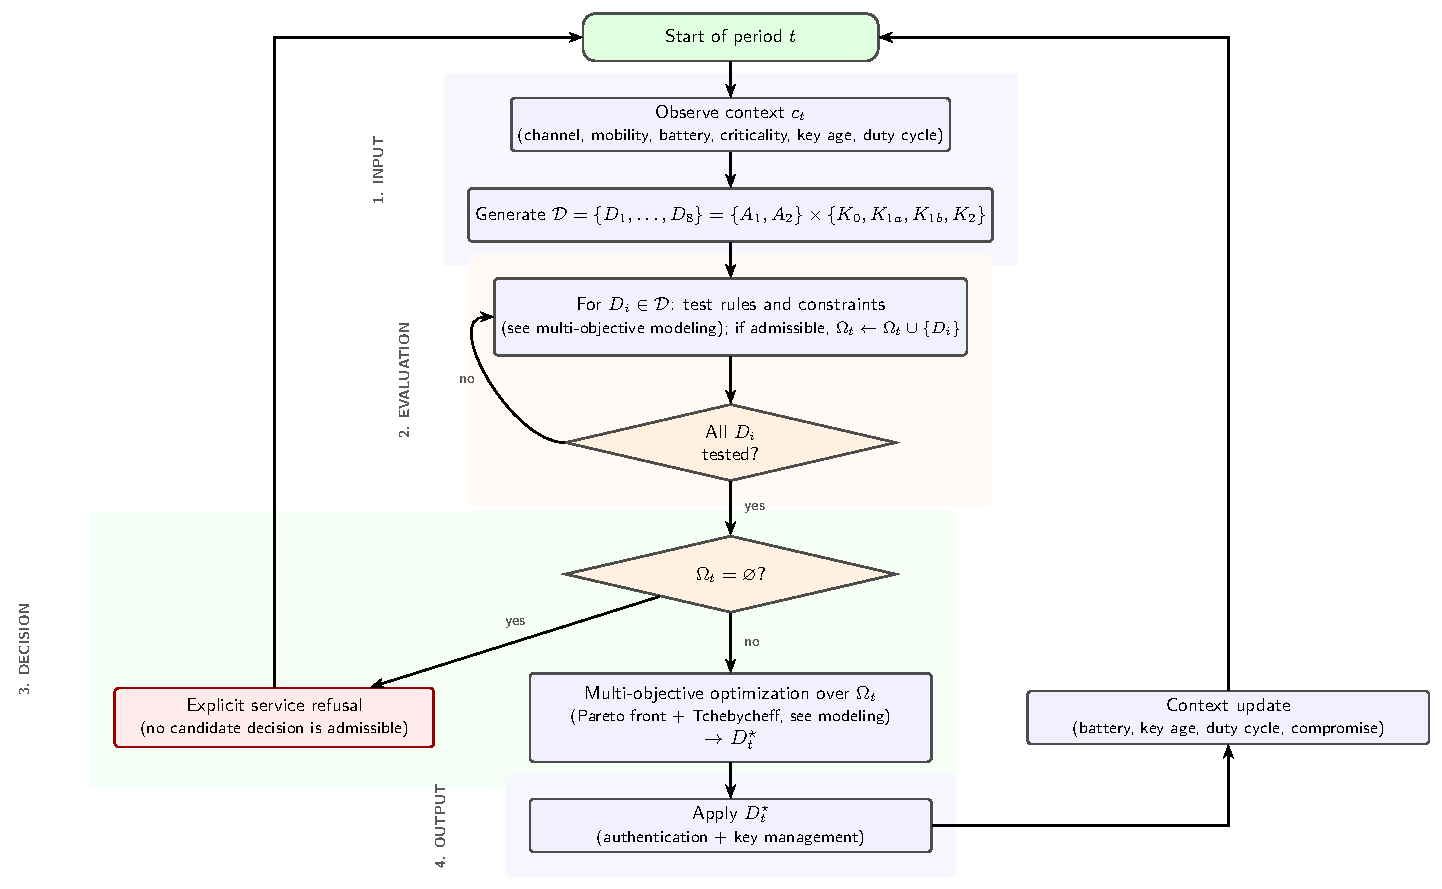
\includegraphics[width=\linewidth]{flowchart_dm_en.pdf}
\caption{Decision flow of P0. The context is observed, the eight candidate decisions are generated, admissibility rules are tested, the Pareto front is built, and the Tchebycheff scalarization selects the applied decision.}
\label{fig:model}
\end{figure}

\section{Methodology}
\label{sec:methodology}

\subsection{Energy Transposition}

The energy of the hybrid scheme is modelled as an aggregate calibrated on the four published points. The RFF-only value supplies the per-message base cost $E_{\mathrm{RFF}}$. A $2\times2$ linear system on the two hybrid points yields two effective parameters: a fixed hybrid overhead $F$ and a per-fallback cost $C$,
\begin{equation}
  E_{\mathrm{hybrid}}(\mathrm{FRR}) = E_{\mathrm{RFF}} + F + N \cdot \mathrm{FRR} \cdot C,
\end{equation}
with $N=100$ messages. All four published values are reproduced by construction. Parameter $F$ is not presented as the physical cost of the initial authentication, but as an aggregate that may absorb it. The calibration is therefore an adjustment to published points, not an independent validation.

\subsection{Published RFF Performance}

When P0 evaluates the RFF candidate, it receives the security performance measured by Haenel et al.\ (FAR$=0.002$). It does not receive the FAR of an internal channel model, which depends on an assumed signal-to-noise ratio that has never been published for this testbed. The published value is injected before scalarization, and the FAR of the candidate is composed with the decision engine's own formula. The internal-channel variant is kept as a separate sensitivity analysis and is never mixed with the main comparison.

\subsection{Correction of the Scalarization}

In an earlier implementation, a small numerical constant was added to every normalization denominator of the Tchebycheff score, including non-degenerate ones. This shifted the scores of the candidates by about $2.5\times10^{-11}$, a value larger than the tolerance used to detect ties. In roughly one third of the tested periods with equal weights, the FAR-first tie-break was thereby bypassed. The constant is now used only to detect a numerically null span. The defect was identified during this work and corrected. All scenario results reported below come from the corrected campaign. Results obtained with the earlier implementation are not reported. The Haenel-calibrated comparison was computed with the corrected implementation.

\subsection{Bottom-Up Structural Model}

An event-driven TX/RX/CPU energy model is also built from the official datasheets of the MSP430G2x and CC110L components. Unpublished parameters (frame size, data rate, Chaskey cycle cost, calibration time) are varied over documented low, central and high ranges. The model is evaluated on the incremental overhead above the RFF-only baseline, because that baseline is reproduced by construction and would otherwise inflate the apparent explanatory power.

\subsection{Experimental Scenarios}
\label{sec:scenarios}

Three experimental settings are used.

\textbf{Experiment A (Haenel transposition).} This setting adapts the energy testbed of Haenel et al.~\cite{haenel2021practical}: 300~s, 100 messages, FRR of 5\% and 10\%, two candidates (RFF and MAC), and the published FAR of 0.002. Only the two candidates of the original scheme are retained. The calibrated values of Section~\ref{sec:methodology} are used, and 30 Monte Carlo seeds are simulated for the calibrated fallback policy (B5\_HAENEL\_CALIBRATED).

\textbf{Dedicated security campaign.} Each policy is attacked with 100{,}000 Bernoulli trials. Exact Clopper--Pearson 95\% intervals are reported.

\textbf{Five adaptive scenarios (S1 to S5).} These scenarios are defined in the simulator and are not taken from another publication. They vary the deployment context, as summarized in Table~\ref{tab:scenarios}. S1 is an isolated agricultural sensor with a single phase. S2 is an industrial critical alarm with a normal, an alarm and a recovery phase. S3 is an object carried by a vehicle that stops, accelerates, cruises at up to 30~km/h, decelerates and stops. S4 is a dense urban network alternating normal and congestion phases. S5 is a critical infrastructure under attack, with a normal phase, a compromise phase with a high attack probability, and a recovery phase. Each scenario is simulated with common random numbers across policies. The number of seeds follows an adaptive stopping rule bounded between 30 and 150 seeds. Four reference policies are compared with P0. B1 is the conventional policy, which always uses cryptography. B2 is a naive physical-layer policy with a fixed preference and no FAR floor. B3 is the fixed hybrid rule, with a FAR floor and no fallback search. B4 is the same decision maker as P0 without the FAR floor, and it isolates the effect of that floor.

\begin{table}[t]
\centering
\caption{Configuration of the five adaptive scenarios (corrected campaign).}
\label{tab:scenarios}
\begin{tabular}{lccccc}
\toprule
 & S1 & S2 & S3 & S4 & S5 \\
\midrule
Node & fixed & fixed & mobile & fixed & fixed \\
Mean SNR (dB) & 8 & 6 & 9--10 & 3 & 12 \\
Attack probability & 0.10 & 0.15 & 0.10 & 0.20--0.30 & 0.10--0.50 \\
Separation factor & 4.0 & 2.0 & 2.0 & 1.0 & 0.5 \\
CPU-cost profile & LOW & HIGH & CENTRAL & CENTRAL & HIGH \\
\bottomrule
\end{tabular}
\end{table}

\section{Results and Discussion}
\label{sec:results}

\subsection{Haenel-Calibrated Comparison}

Figure~\ref{fig:story} compares the published energy of Haenel et al.\ with the calibrated fallback policy and with P0. The published hybrid energy decreases as the FRR falls. The calibrated policy follows the same trend, and its 95\% confidence band is shown. P0 keeps a constant energy level at the MAC-only ceiling, whatever the FRR. Under equal weights, P0 therefore costs 24.4\% more than the hybrid rule at FRR=10\%, and 39.5\% more at FRR=5\%. The FRR=5\% comparison carries an assumed FAR, as explained in the limits below. Figure~\ref{fig:split} shows the decision mix message by message. The hybrid rule mixes RFF and MAC messages in proportion to the FRR, whereas P0 selects the MAC path for every message.

\begin{figure}[t]
\centering
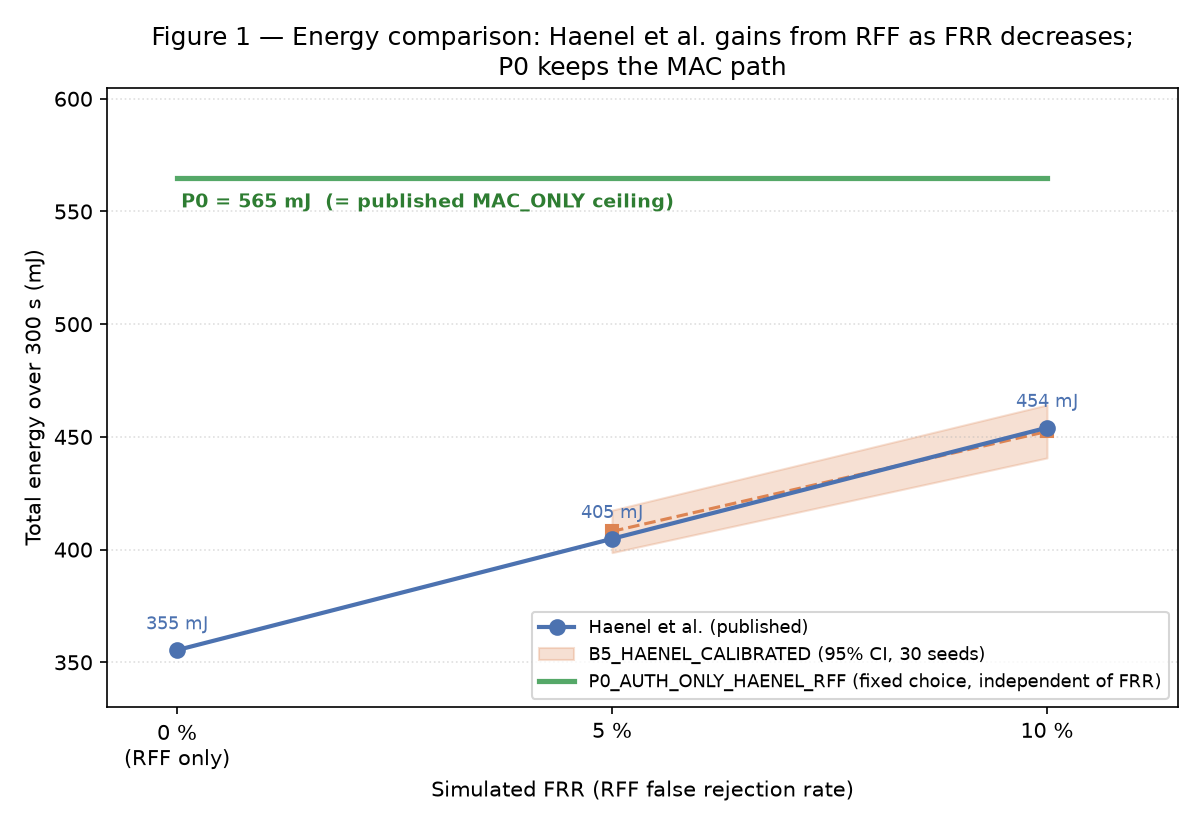
\includegraphics[width=\linewidth]{figure_1_energy_comparison_en.png}
\caption{Calibrated energy as a function of the simulated FRR. The hybrid rule decreases with the FRR. P0 stays flat at the MAC-only ceiling.}
\label{fig:story}
\end{figure}

\begin{figure}[t]
\centering
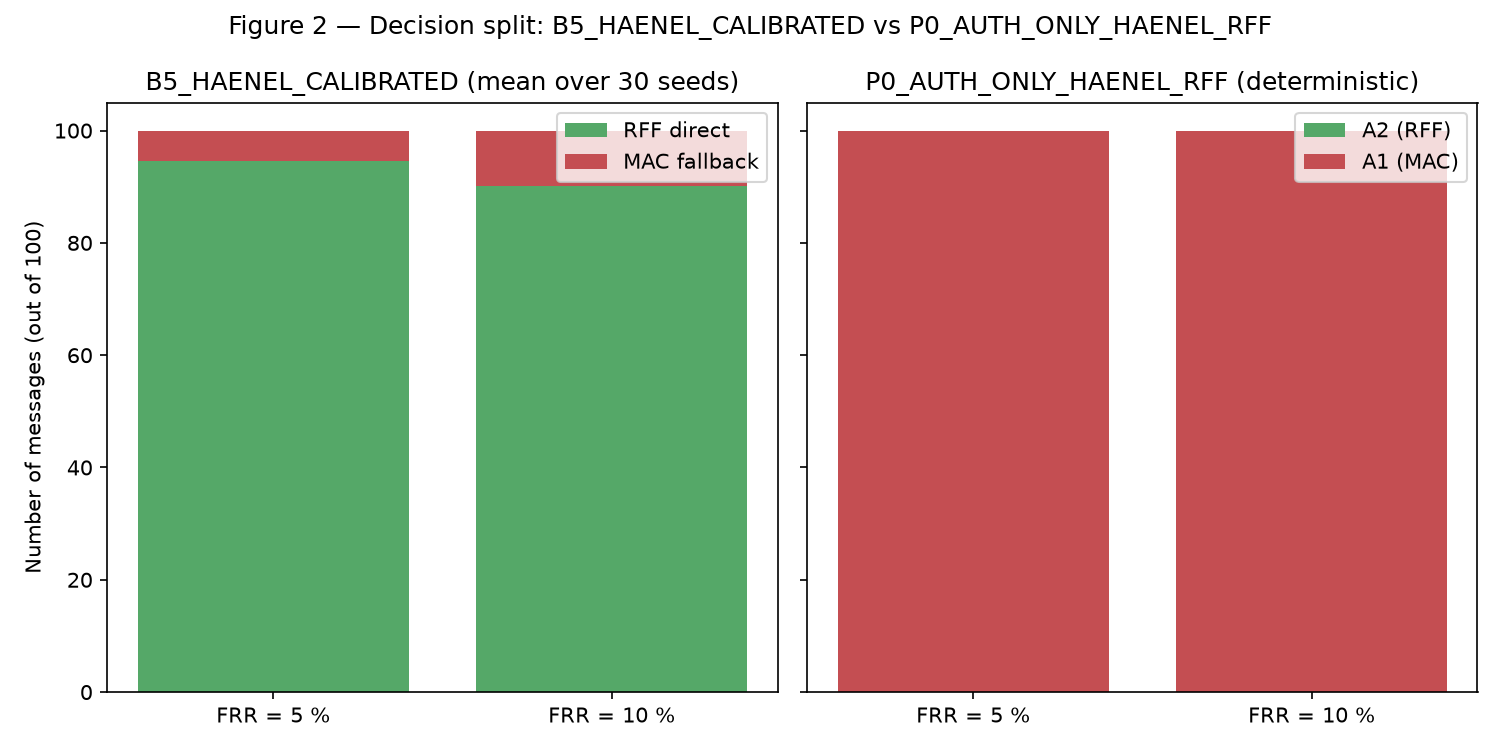
\includegraphics[width=\linewidth]{figure_2_decision_split_en.png}
\caption{Decision split per 100 messages at FRR=5\% and 10\%. The hybrid rule alternates between RFF and MAC, while P0 selects MAC for all messages.}
\label{fig:split}
\end{figure}

\subsection{Why P0 Stays on the MAC Path: An Exact Tie}

With key management fixed and latency neutralized on both sides, the Pareto front reduces to two points. Each point is ideal on one objective and at the nadir on the other. Equation~\eqref{eq:tcheby} then reduces to
\begin{equation}
  s(\text{MAC}) = w_{\mathrm{energy}}, \qquad
  s(\text{RFF}) = w_{\mathrm{auth}}.
\end{equation}
The MAC is therefore preferred when $w_{\mathrm{energy}} < w_{\mathrm{auth}}$, the RFF when the inequality is reversed, and equal weights give an exact tie. The tie is resolved by FAR. The analytical prediction was verified by a sweep of 11 weight pairs around $w_{\mathrm{energy}}=w_{\mathrm{auth}}=0.25$ (Table~\ref{tab:boundary}, Fig.~\ref{fig:boundary}). The maximum discrepancy between predicted and computed scores is $0$ to machine precision. A weight shift of 0.001 reverses the decision.

\begin{table}[t]
\centering
\caption{Weight boundary sweep (fixed case: FRR=10\%, FAR=0.002).}
\label{tab:boundary}
\begin{tabular}{ccccc}
\toprule
$w_{\mathrm{energy}}$ & $w_{\mathrm{auth}}$ & $s(\mathrm{MAC})$ & $s(\mathrm{RFF})$ & Choice \\
\midrule
0.245 & 0.255 & 0.245 & 0.255 & MAC \\
0.249 & 0.251 & 0.249 & 0.251 & MAC \\
\textbf{0.250} & \textbf{0.250} & \textbf{0.250} & \textbf{0.250} & MAC (tie-break) \\
0.251 & 0.249 & 0.251 & 0.249 & \textbf{RFF} \\
0.255 & 0.245 & 0.255 & 0.245 & RFF \\
\bottomrule
\end{tabular}
\end{table}

\begin{figure}[t]
\centering
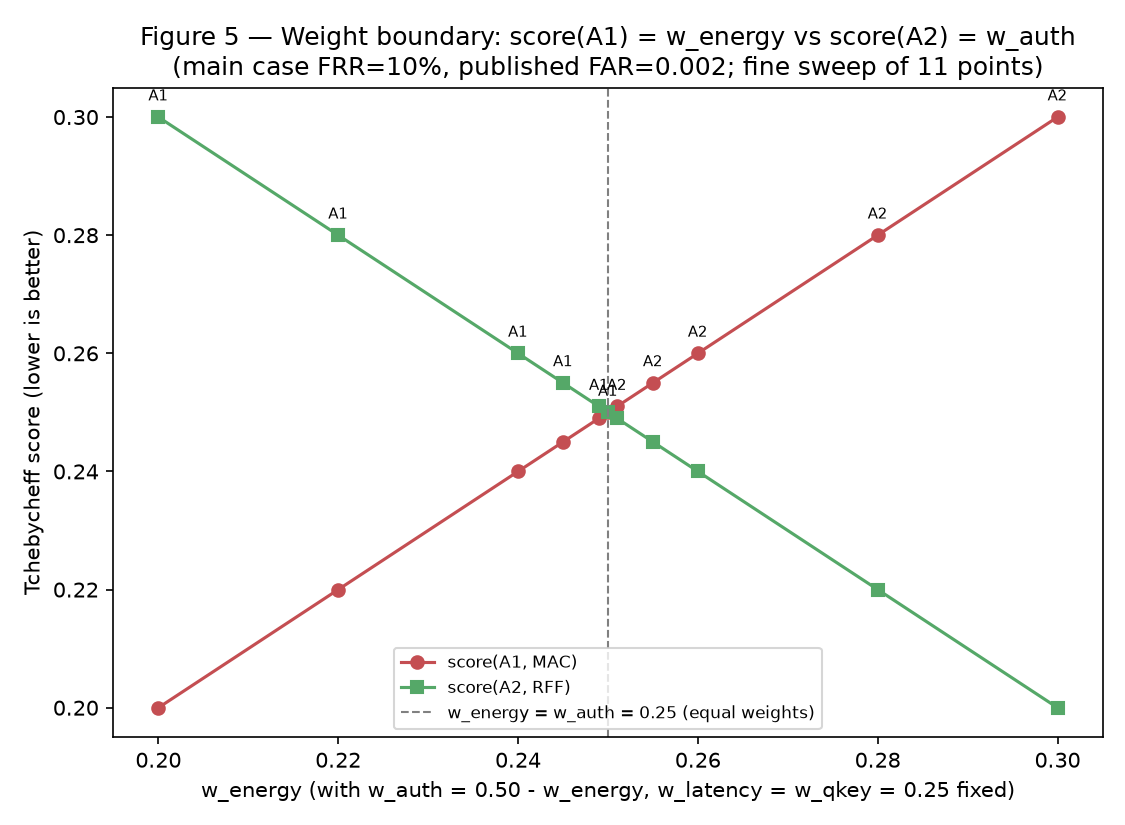
\includegraphics[width=\linewidth]{figure_5_weight_sensitivity_en.png}
\caption{Tchebycheff scores of MAC and RFF as functions of $w_{\mathrm{energy}}$ over the 11-point sweep. The two curves cross exactly at $w_{\mathrm{energy}}=w_{\mathrm{auth}}=0.25$.}
\label{fig:boundary}
\end{figure}

This boundary is a sensitivity result, not a finding of strong security preference. A reader who sets the weights slightly differently obtains the RFF choice. The energy saving of the RFF path is real, but at equal weights it is exactly balanced by the robustness advantage of the MAC.

\subsection{Security Campaign}

The initial campaign of 30 seeds, with about 450 attack attempts, was too small to estimate a FAR of 0.2\%. A dedicated campaign of 100{,}000 trials per policy was therefore run. The RFF path accepts 189 of 100{,}000 attempts (0.189\%, $\mathrm{CI}_{95}=[0.163\%,0.218\%]$), which is consistent with the published 0.2\%. The MAC path of P0 accepts 0 of 100{,}000 attempts. Its 95\% upper bound, $3.7\times10^{-5}$, is larger than the theoretical bound of the model, $5.4\times10^{-20}$. This campaign therefore cannot separate the two values. It is not presented as experimental proof of superior security.

\begin{figure}[t]
\centering
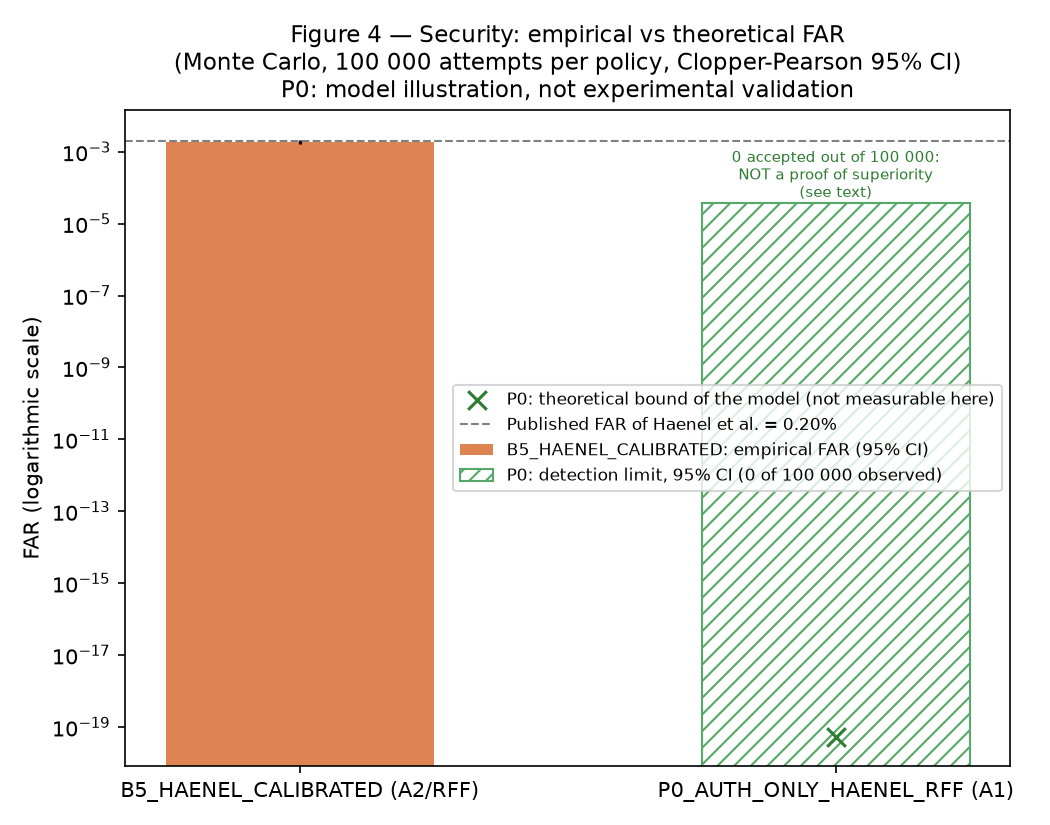
\includegraphics[width=\linewidth]{figure_4_security_en.png}
\caption{Empirical FAR of the RFF path with Clopper--Pearson 95\% intervals, against the published 0.2\% target, and the MAC path of P0 with zero acceptances over 100{,}000 trials. The upper bound of the interval is shown.}
\label{fig:security}
\end{figure}

\subsection{Overhead Explained by the Bottom-Up Model}

The incremental energy of the bottom-up model above the RFF-only baseline is compared with the same quantity in the published data. The explained fraction ranges from 0.19\% (low assumptions) to 14.45\% (high assumptions, MAC-only case). The qualitative ordering of the four configurations is reproduced under every assumption set. The magnitude is not reproduced. A substantial part of the real overhead, plausibly an unquantified listening window or resynchronization cost, is not explained by public datasheets.

\subsection{Five Adaptive Scenarios}

Table~\ref{tab:scen} summarizes the comparison of P0 with the reference policies in the corrected campaign. Energy and latency are averaged over the periods that each policy serves, and the energy of a policy that refuses requests is therefore computed on fewer periods. Figures~\ref{fig:s2} and \ref{fig:s4} show the four objectives for the two scenarios where the reference policies differ most.

\begin{table*}[t]
\centering
\caption{Comparison of P0 with the reference policies in the five scenarios (corrected campaign; means over seeds).}
\label{tab:scen}
\begin{tabular}{lccccc}
\toprule
 & S1 & S2 & S3 & S4 & S5 \\
\midrule
Seeds & 30 & 120 & 40 & 90 & 150 \\
Attacker attempts & 4{,}426 & 26{,}978 & 5{,}959 & 31{,}234 & 54{,}131 \\
Accepted attacks, P0 (count) & 0 & 0 & 0 & 0 & 0 \\
Accepted attacks, B2 (\%) & 0 & 12.6 & 1.1 & 70.6 & 55.2 \\
Accepted attacks, B3 (\%) & 0 & 0.4 & 0.1 & 0.04 & 0 \\
Energy saving vs B1 (\%) & 2.8 & 0.08 & 0.02 & 0.02 & 6.9 \\
Energy premium vs B2 (\%) & 2.1 & 3.9 & 4.8 & 4.8 & 4.1 \\
Latency, P0 / B1 (objective) & 0.0015 / 0.0019 & 0.0050 / 0.0050 & 0.0019 / 0.0019 & 0.0020 / 0.0019 & 0.053 / 0.0035 \\
Key quality, P0 / B1 & 0.730 / 0.731 & 0.730 / 0.731 & 0.731 / 0.731 & 0.731 / 0.731 & 0.669 / 0.745 \\
Service rate, P0 (\%) & 100 & 100 & 100 & 100 & 100 \\
Service rate, B1 (\%) & 100 & 100 & 100 & 100 & 94.8 \\
Service rate, B3 (\%) & 99.99 & 38.8 & 44.1 & 2.5 & 0.05 \\
\bottomrule
\end{tabular}
\end{table*}

\begin{figure}[t]
\centering
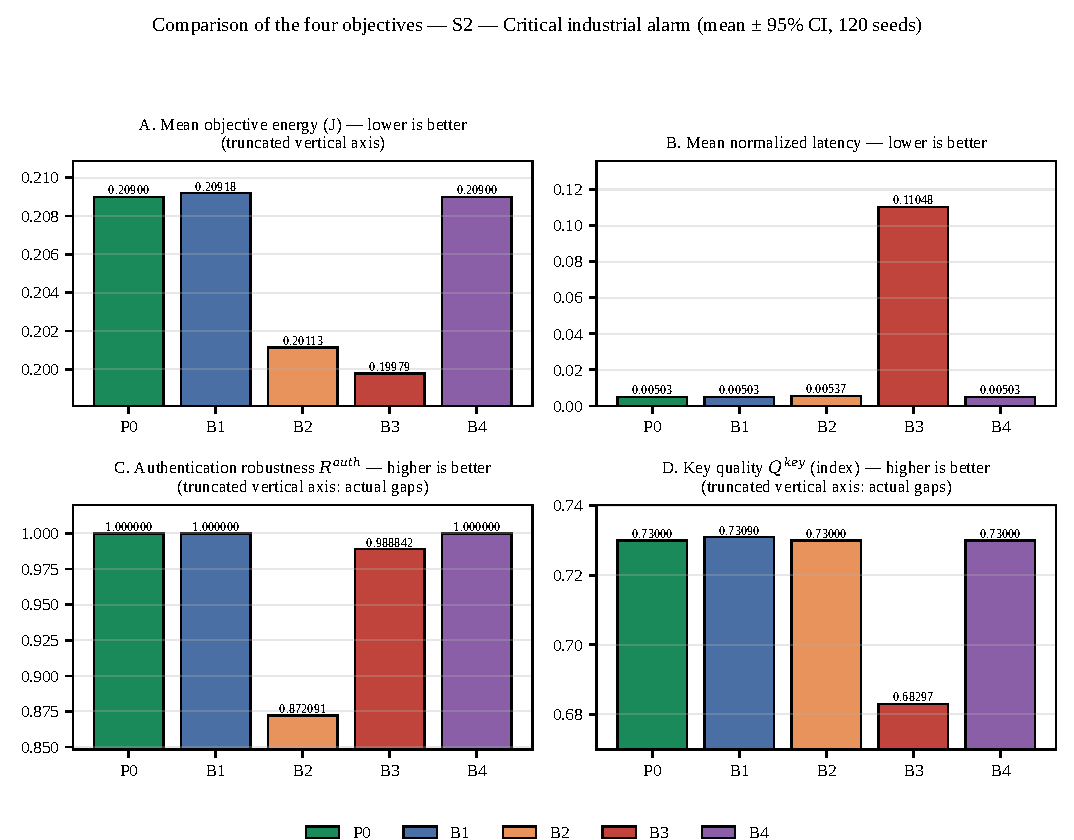
\includegraphics[width=\linewidth]{figure_s2_four_objectives_en.pdf}
\caption{Four objectives for S2 (industrial critical alarm, 120 seeds). B2 accepts 12.6\% of the attacker attempts, against none for P0. B3 serves 38.8\% of the requests.}
\label{fig:s2}
\end{figure}

\begin{figure}[t]
\centering
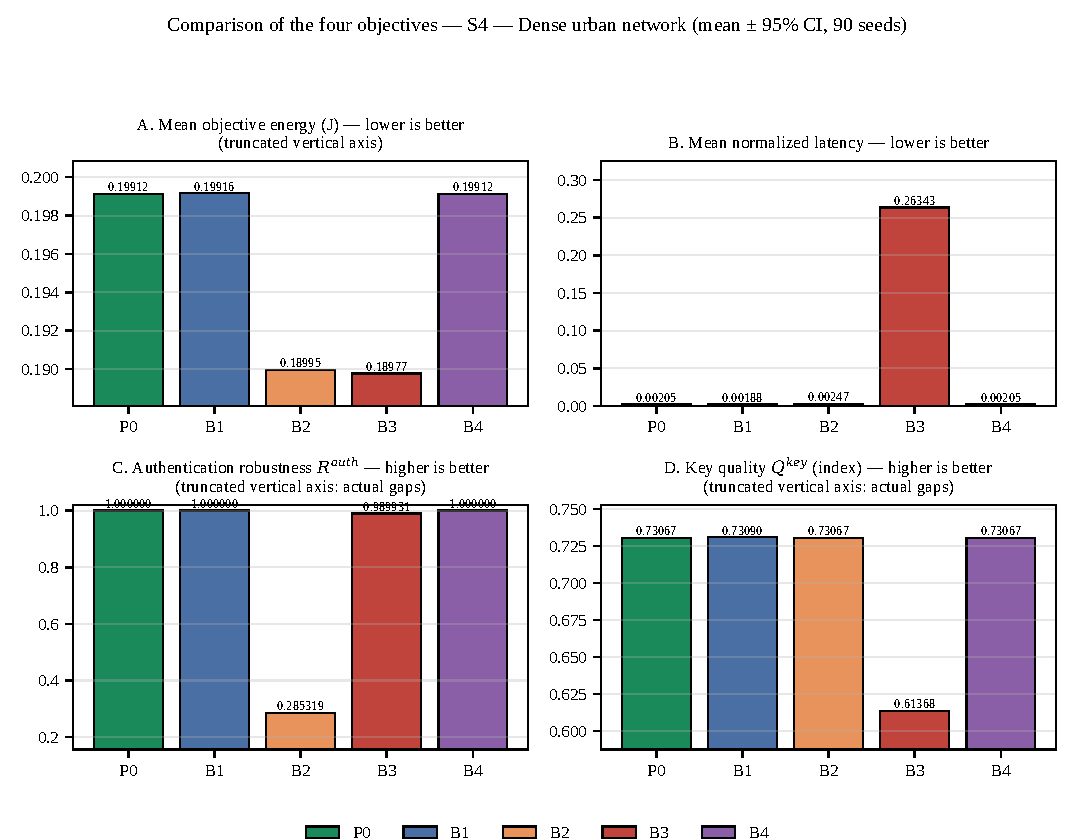
\includegraphics[width=\linewidth]{figure_s4_four_objectives_en.pdf}
\caption{Four objectives for S4 (dense urban network, 90 seeds). B2 accepts 70.6\% of the attacker attempts, with a robustness of 0.285. B3 serves 2.5\% of the requests.}
\label{fig:s4}
\end{figure}

\subsection{Where P0 Performs Better, and Where It Does Not}

P0 never accepts an attack in the five scenarios, and it never refuses a request. Its acceptance count is zero out of 4{,}426 to 54{,}131 attempts, so its 95\% upper bound is about $3/N$, that is at most $5.5\times10^{-5}$ for S5. The naive physical-layer policy B2 accepts between 1.1\% and 70.6\% of the attacks in S2 to S5, and its robustness falls to 0.285 in S4. The fixed hybrid rule B3 serves only 2.5\% of the requests in S4 and 0.05\% in S5. Against the conventional policy B1, P0 saves 2.8\% of energy in S1 and 6.9\% in S5. In S5, B1 refuses 5.2\% of the requests, so its energy average covers fewer periods and is not strictly comparable.

P0 does not perform better on every metric. Its energy is 2.1\% to 4.8\% higher than that of B2, which accepts attacks freely. In S4, the latency of P0 is 9\% higher than that of B1. In S5, P0 has a latency of 0.053 against 0.0035 for B1, and a key quality of 0.669 against 0.745. In that scenario, P0 shares these penalties with B2, which has the same latency and key quality. The energy saving against B1 in S2 to S4 is below 0.1\%. It is statistically distinguishable from zero in the paired analysis, but it is too small to matter in practice.

\subsection{Limits}

Several limits constrain these results. The energy values come from a calibrated model, and the CPU parameters are still awaiting hardware measurement. The mean energy varies by about 8\% between the low and high CPU-parameter profiles. This variation is not large enough to reverse the qualitative comparisons, but it affects the percentages reported above. The channel is simulated, and no radio measurement is used. The weights of P0 are equal by construction, and no contextual weight set has been validated. The S5 campaign did not reach the pre-registered precision within its cap of 150 seeds. The two-candidate analysis of Experiment A is a reduced case, and its conclusions about the decision boundary do not transfer directly to the five-scenario setting.

\section{Conclusion}

A multi-objective decision maker is compared with a fixed fallback rule and with three further policies under explicit security floors. In the corrected campaign, P0 accepts no attack and serves every request in the five scenarios. It saves energy against conventional cryptography in S1 and S5 only. It pays a moderate energy premium over a naive physical-layer policy that accepts attacks, and a latency and key-quality penalty in S5. In the reduced Haenel-calibrated case, the equal-weight decision lies on an exact tie. Future work includes measuring the CPU and radio parameters on hardware, validating a contextual weight set, and extending the comparison to dynamic channels.

\section{Implementation}

The simulator, the calibration scripts, the test suite and the instructions to regenerate every figure and table are available at \url{https://github.com/guygnyolparfait/physec-dm-p0-haenel}. The repository is kept private during preparation and is made public at the end of the work.

\begin{thebibliography}{11}

\bibitem{haenel2021practical}
A.~Haenel, Y.~Haddad, M.~Laurent, and Z.~Zhang, ``Practical cross-layer radio frequency-based authentication scheme for internet of things,'' \emph{Sensors}, vol.~21, no.~12, p.~4034, 2021.

\bibitem{das2018deep}
R.~Das, A.~Gadre, S.~Zhang, S.~Kumar, and J.~M.~F. Moura, ``A deep learning approach to IoT authentication,'' in \emph{Proc. IEEE Int. Conf. Communications (ICC)}, 2018.

\bibitem{baldini2017physical}
G.~Baldini, R.~Giuliani, G.~Steri, and R.~Neisse, ``Physical layer authentication of Internet of Things wireless devices through permutation and dispersion entropy,'' in \emph{Proc. IEEE Global Internet of Things Summit (GIoTS)}, 2017.

\bibitem{nouichi2019iot}
D.~Nouichi, M.~Abdelsalam, Q.~Nasir, and S.~Abbas, ``IoT devices security using RF fingerprinting,'' in \emph{Proc. IEEE Int. Conf. Advances in Science and Engineering Technology (ASET)}, 2019.

\bibitem{merchant2019enhanced}
K.~Merchant and B.~Nousain, ``Enhanced RF fingerprinting for IoT devices with recurrent neural networks,'' in \emph{Proc. IEEE Military Communications Conf. (MILCOM)}, 2019, pp.~590--597.

\bibitem{wilson2019integration}
A.~J. Wilson, D.~R. Reising, and T.~D. Loveless, ``Integration of matched filtering within the RF-DNA fingerprinting process,'' in \emph{Proc. IEEE Global Communications Conf. (GLOBECOM)}, 2019.

\bibitem{gopalakrishnan2019robust}
S.~Gopalakrishnan, M.~Cekic, and U.~Madhow, ``Robust wireless fingerprinting via complex-valued neural networks,'' presented at \emph{IEEE Global Communications Conf. (GLOBECOM)}, 2019. [Online]. Available: arXiv:1905.09388.

\bibitem{morge2022rf}
L.~Morge-Rollet, F.~Le~Roy, D.~Le~Jeune, C.~Canaff, and R.~Gautier, ``RF eigenfingerprints, an efficient RF fingerprinting method in IoT context,'' \emph{Sensors}, vol.~22, no.~11, p.~4291, 2022.

\bibitem{li2018robust}
X.~Li, J.~Peng, J.~Niu, F.~Wu, J.~Liao, and K.-K.~R. Choo, ``A robust and energy efficient authentication protocol for industrial internet of things,'' \emph{IEEE Internet of Things Journal}, vol.~5, no.~3, pp.~1606--1615, 2018.

\bibitem{prantl2023recommendation}
T.~Prantl, A.~Bauer, L.~Iffl\"ander, C.~Krupitzer, and S.~Kounev, ``Recommendation of secure group communication schemes using multi-objective optimization,'' \emph{Int. J. Information Security}, vol.~22, no.~5, pp.~1291--1332, 2023.

\bibitem{prvulovic2025hermees}
P.~Prvulovic, N.~Radosavljevic, D.~Babic, and D.~Drajic, ``HERMEES: A holistic evaluation and ranking model for energy-efficient systems applied to selecting optimal lightweight cryptographic and topology construction protocols in wireless sensor networks,'' \emph{Sensors}, vol.~25, no.~9, p.~2732, 2025.

\end{thebibliography}

\end{document}
